\section{Analyse de l'existant}
 \subsection{Erco.xyz \cite{Erco}}


Erco est un outil initialement développé à l'Université de Lorraine facilitant la configuration  des routes réseau avec Exabgp en réécrivant une partie du fichier de configuration d'Exabgp. Erco fournit une API RESTful et une interface web utilisateur. L'interface web permet de facilement : annoncer un nouveau réseau ou IP, modifier ou supprimer une route, envoyer des commandes à Exabgp( reload, show routes show neighbors et version)
\\
\\
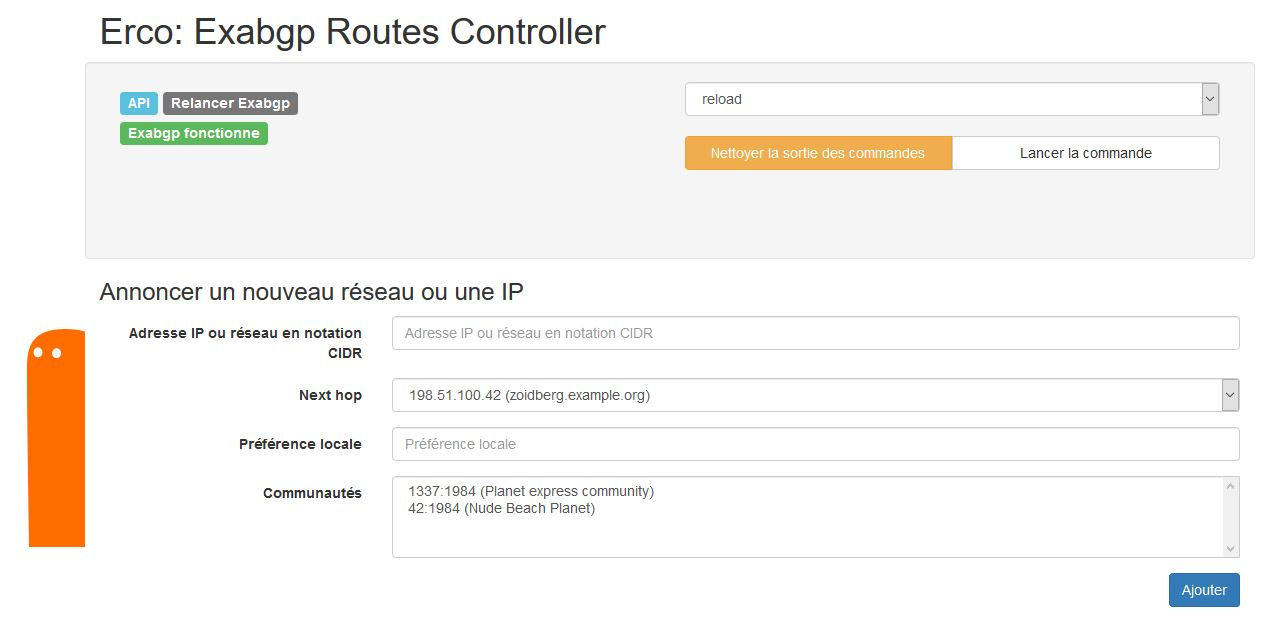
\includegraphics[scale = 0.5]{img/erco1.JPG}
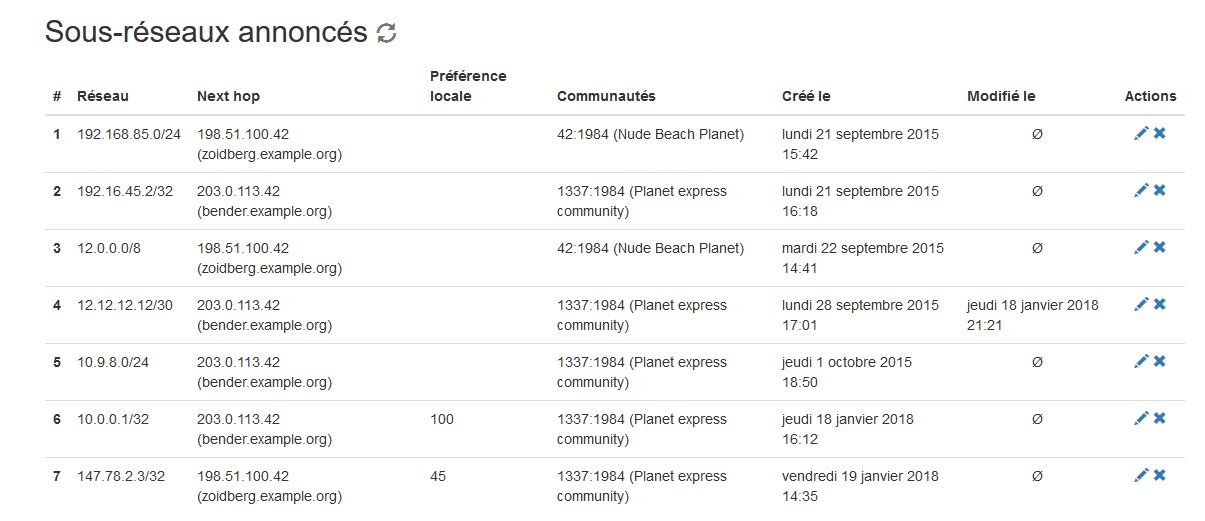
\includegraphics[scale = 0.5]{img/erco2.JPG}

\subsection{ExaBGPmon}

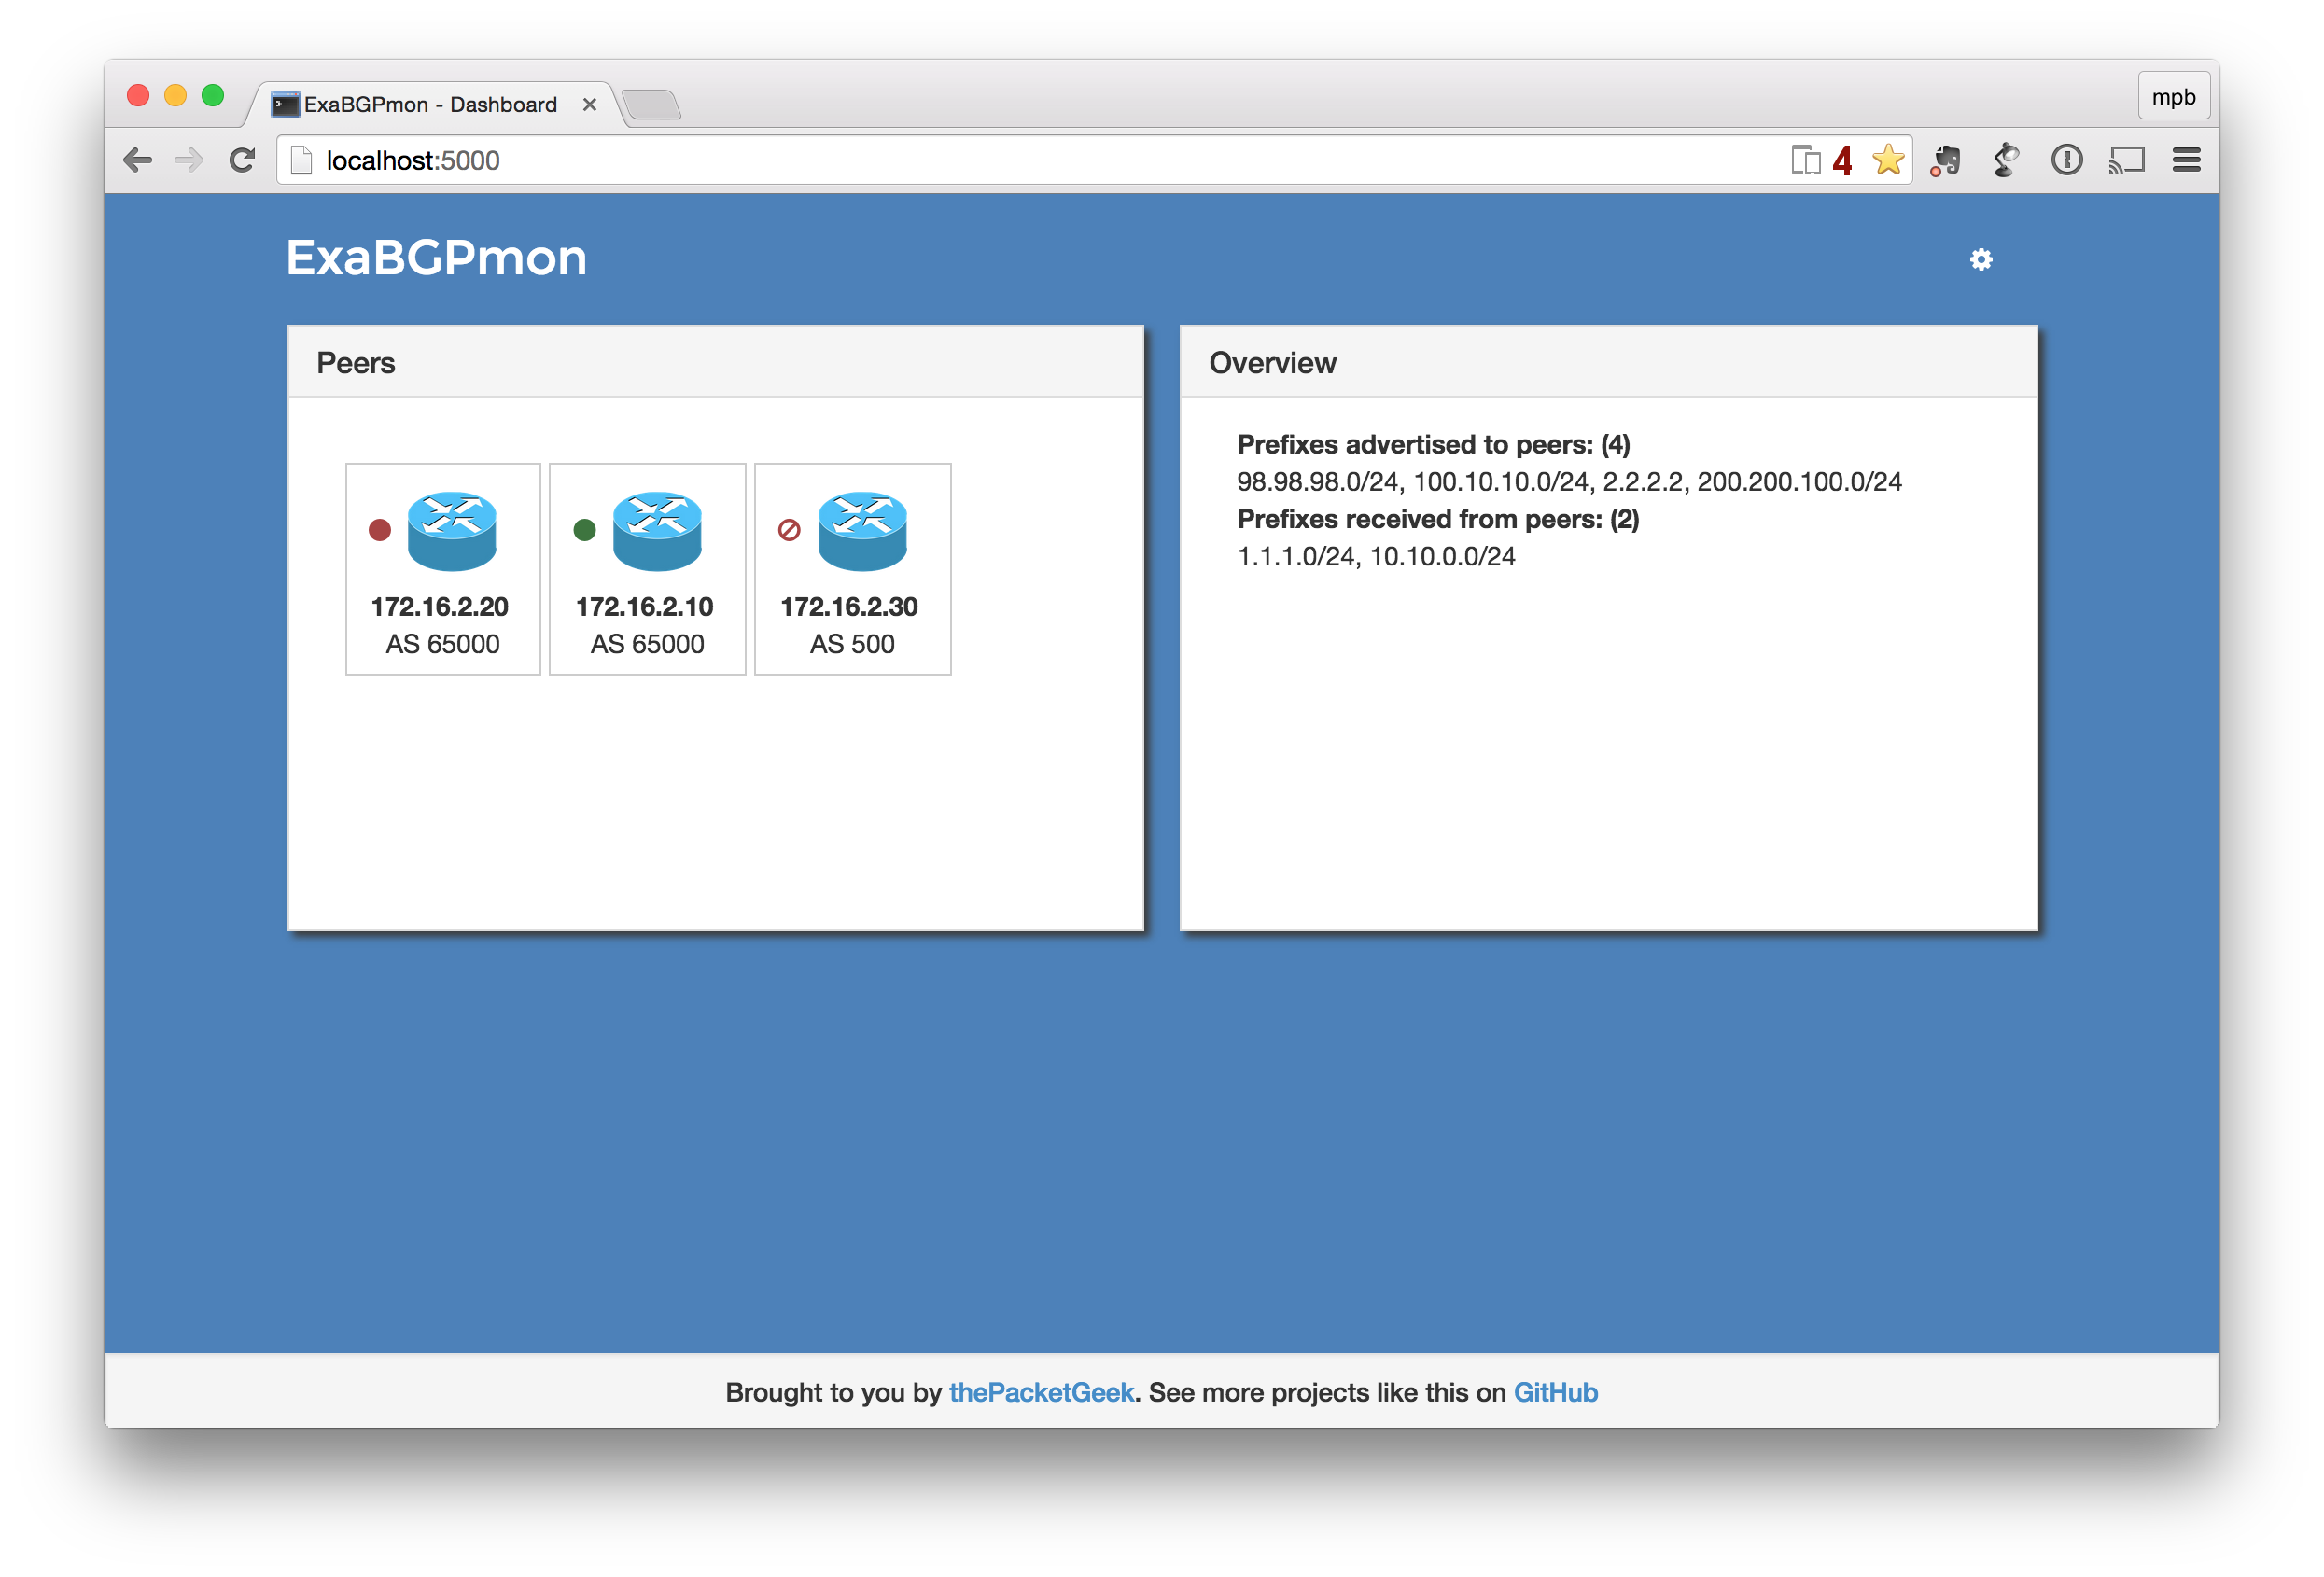
\includegraphics[scale = 0.40]{img/exabgpmon.png}
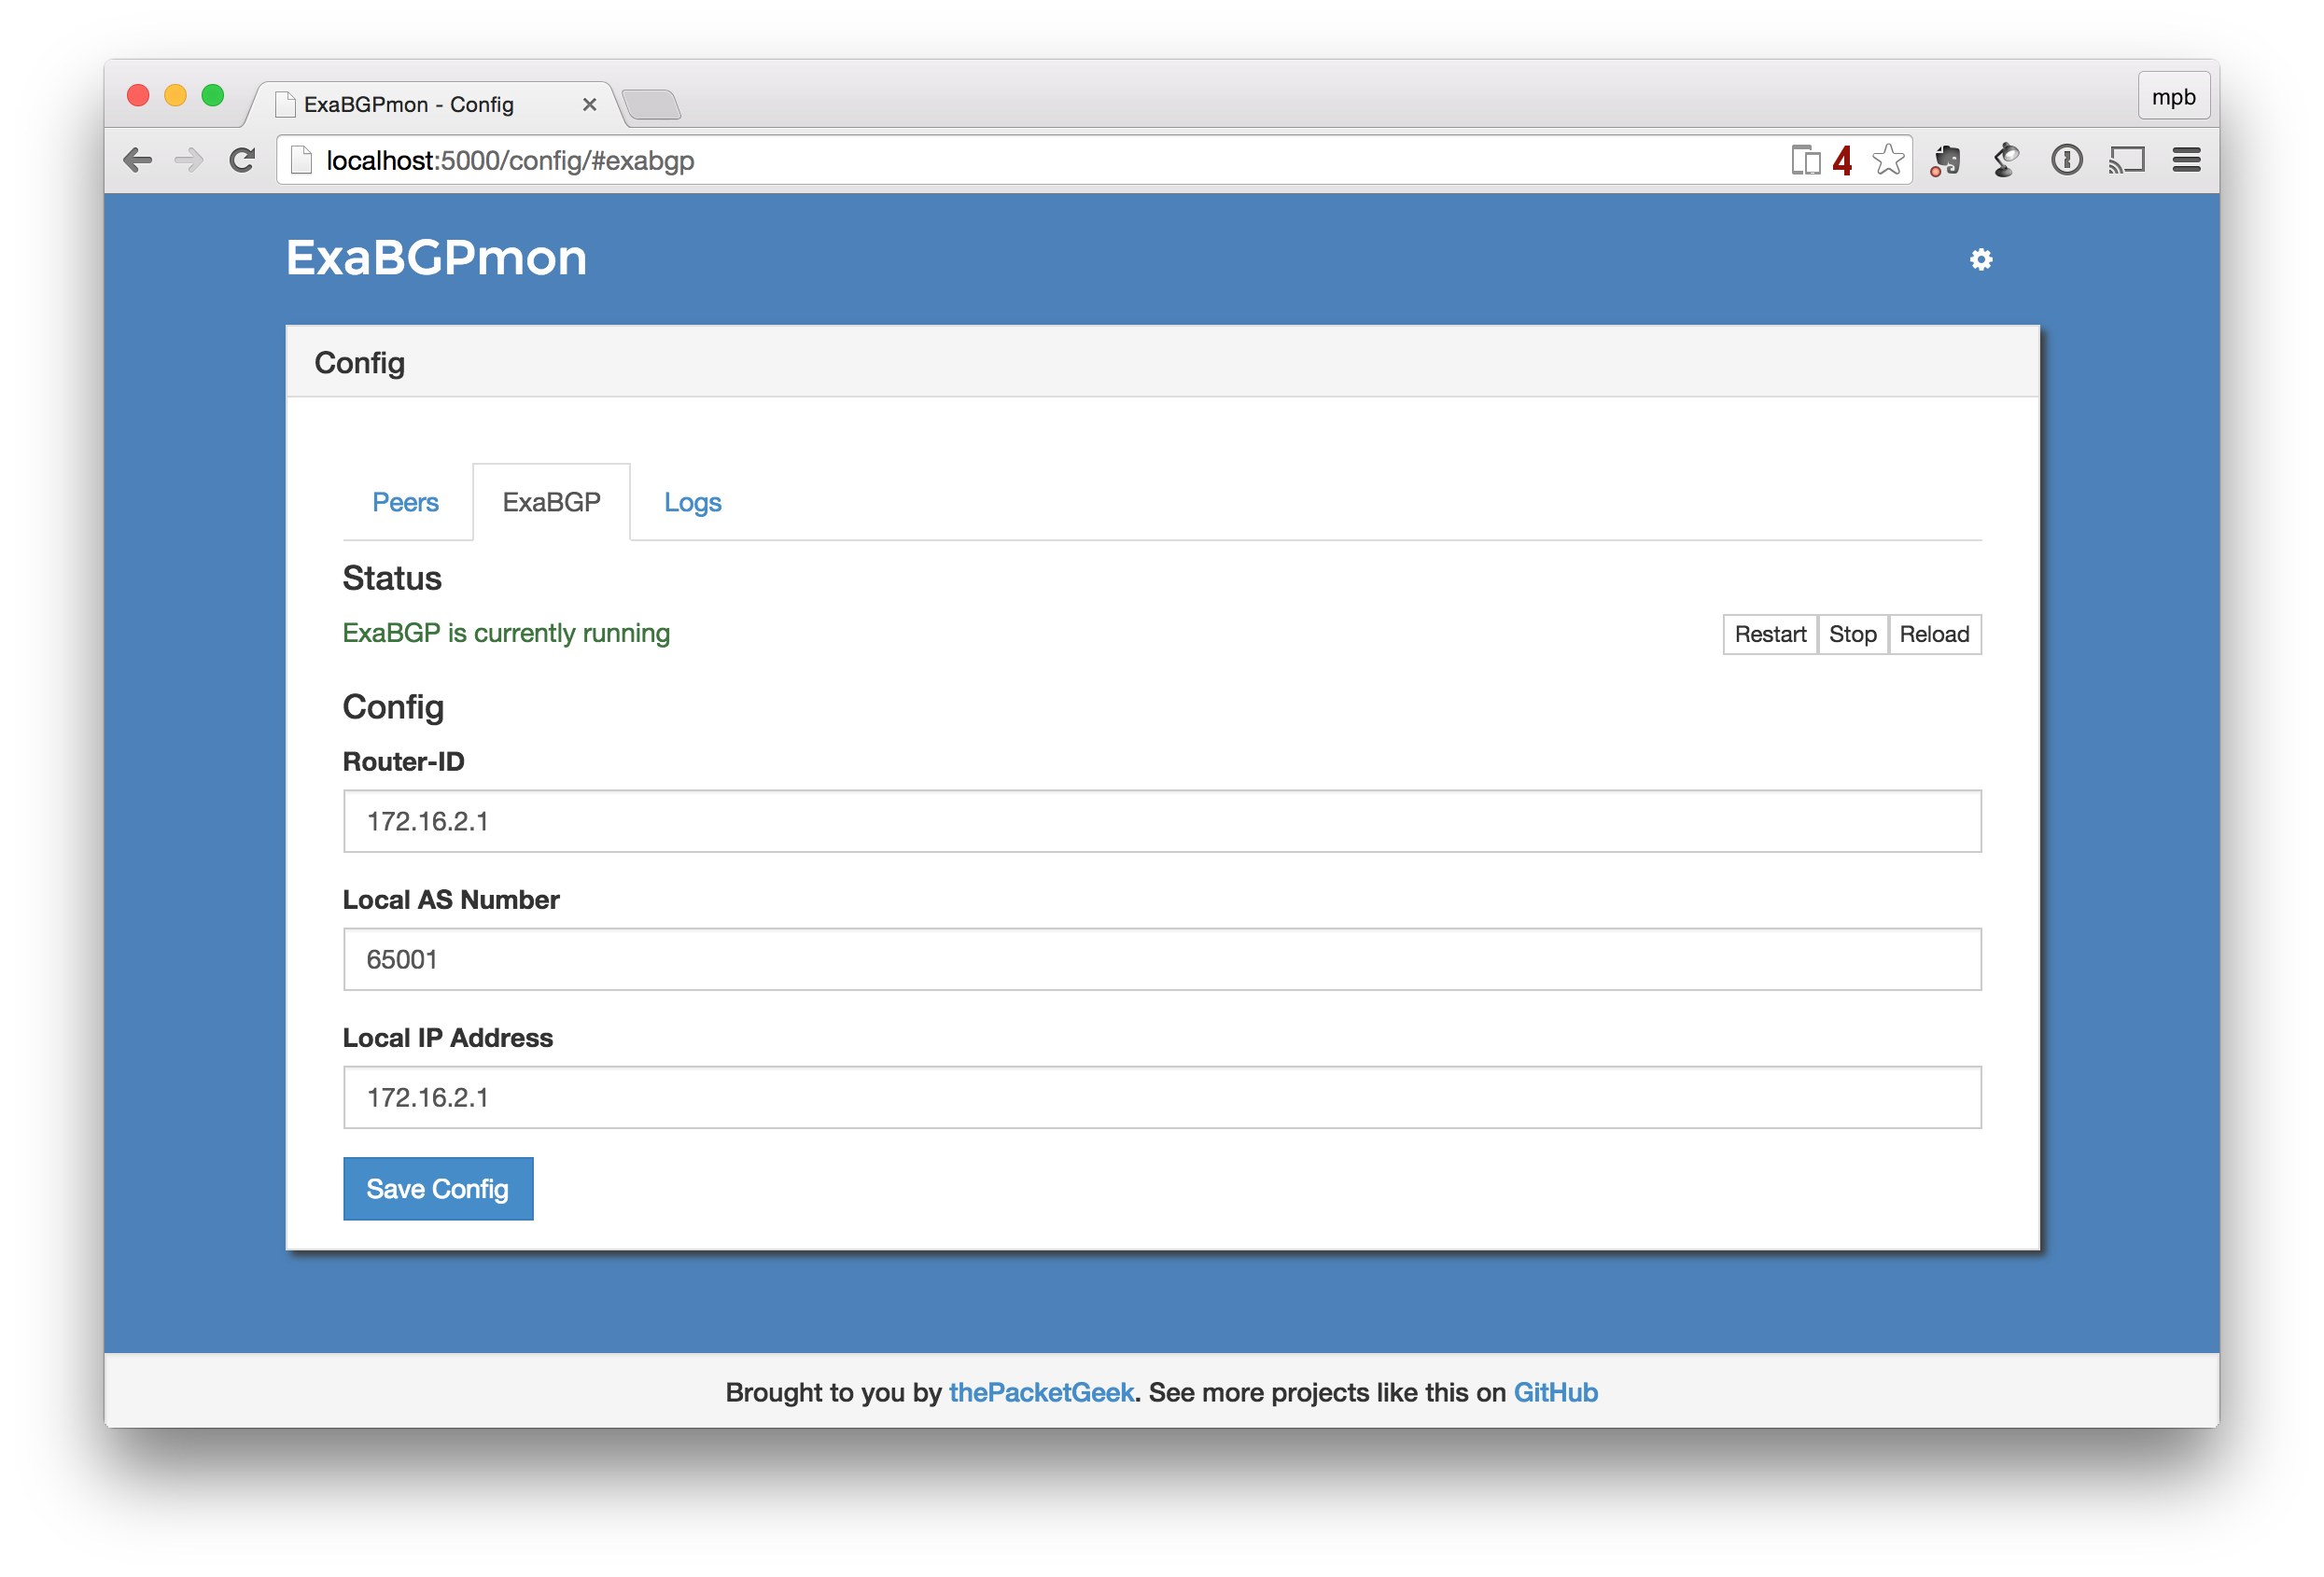
\includegraphics[scale = 0.40]{img/exabgpmon2.png}

\subsection{ExaBGP}
ExaBGP est un outil open source écrit en Python qui permet d'interagir avec les réseaux BGP. Le logiciel peut injecter des routes annoncés dans les réseaux. 
ExaBGP offre un API contenant plusieurs commandes afin de manipuler les routeurs BGP. On peut aller voir la liste des commandes dans l'API d'ExaBGP : 
\\
\\
\url{https://github.com/Exa-Networks/exabgp/wiki/Controlling-ExaBGP-:-interacting-from-the-API}

\subsection{Meteor.JS \cite{Meteor.JS}}
\begin{center}

\includegraphics[height=1cm]{img/Meteor-logo.png}
\end{center}

Meteor.JS est un framework open-source javascript, Node.JS qui permet l'élaboration d'une application web de type RESTful. Elle permet de développer le client et le serveur de l'application web avec le même langage.  

client javascript RESTfull, nous plus facile package, serveur cache client.

